\chapter{Incentives and Truthfulness}
\label{cha:incentives_and_truthfulness}

\begin{figure}
    \centering
    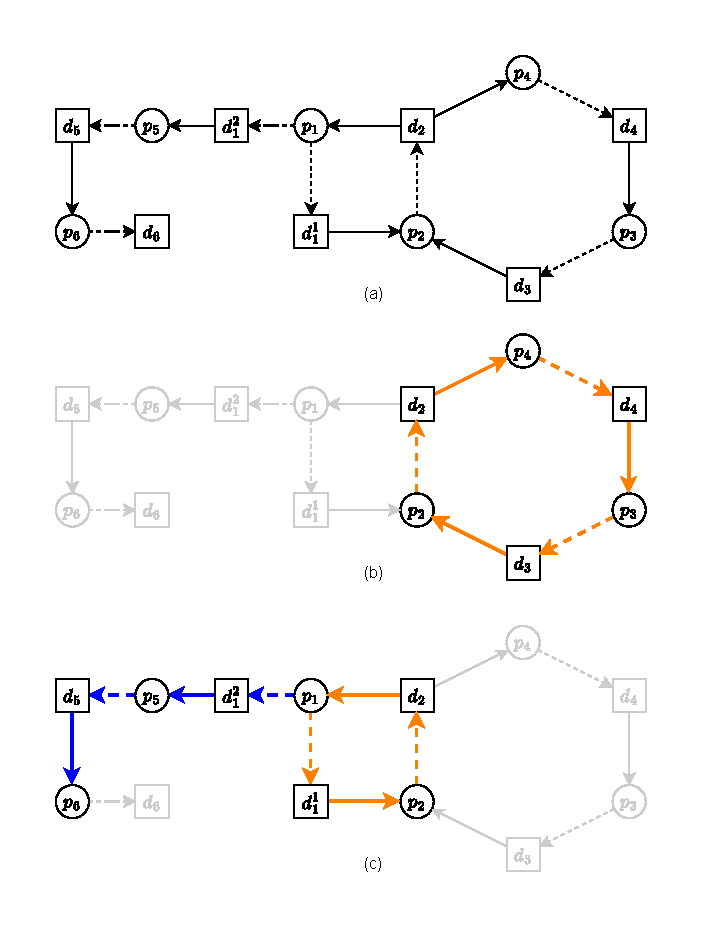
\includegraphics{data/incentive_motivation_example.pdf}
    \caption[An example showing the difference between alternative-donors model and simultaneous-donors model]{\textbf{(a)} shows an example of a graph containing two overlapping cycles, where the left cycle contains patient $p_1$ which has two proxy donors: $d_1^1$ and $d_1^2$. \textbf{(b)} shows the output of the alternative-donors model. \textbf{(c)} shows the output of the simultaneous-donors model.}
    \label{fig:incentive_motivation_example}
\end{figure}


\begin{figure}
    \centering
    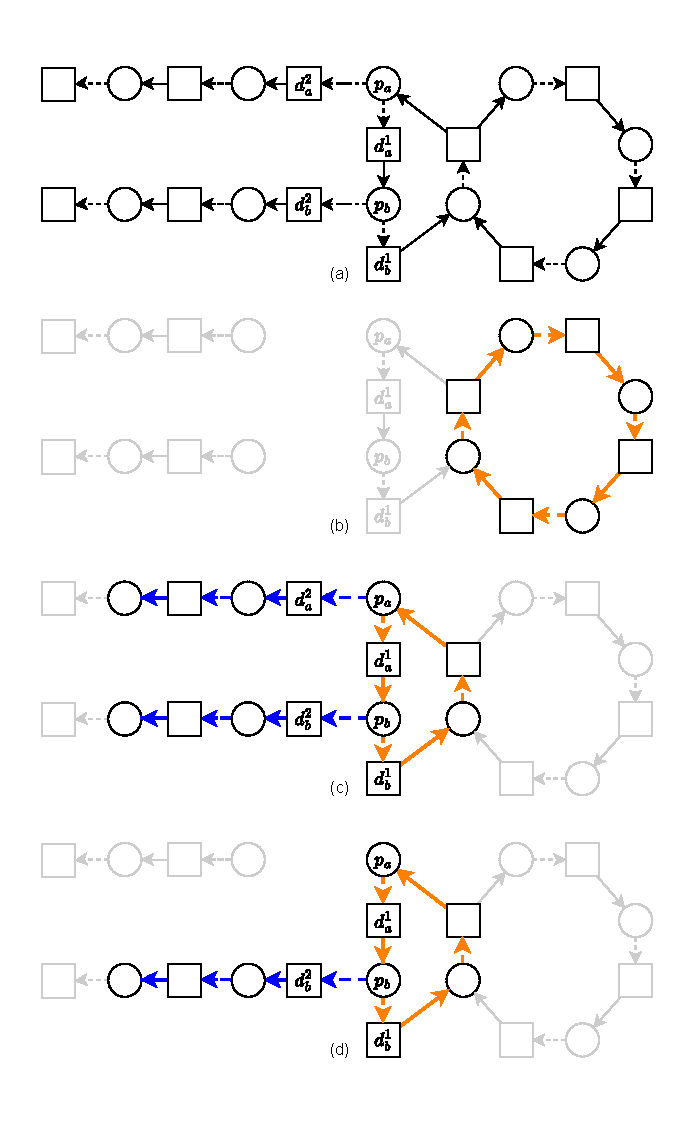
\includegraphics{data/prisoners_dilemma.pdf}
    \caption[Prisoner's dilemma in simultaneous-donors model]{}
    \label{fig:prisoners_dilemma}
\end{figure}


%%% Local Variables:
%%% mode: latex
%%% TeX-master: "../ClassicThesis"
%%% ispell-dictionary: "british" ***
%%% fill-column: 76 ***
%%% End:
